\section{Ejercicio 9}

El algoritmo de $RSDL$ tiene la ventaja de otorgar prioridad a las tareas interactivas a la vez que es ecuánime con la asignación de recursos del CPU. Eventualmente todas las tareas corren, puesto que las cuotas individuales y globales de cada nivel garantizan que, rotaciones mediante, aún los procesos de mayor prioridad alcanzarán el nivel de otros procesos, generando por cierto tiempo una horizontalidad de prioridades.\\
\indent Resulta interesante observar el siguiente gráfico para ilustrar algunos de los conceptos expuestos en el Ejercicio 5.

\begin{figure}[h]
	\centering                                                       
	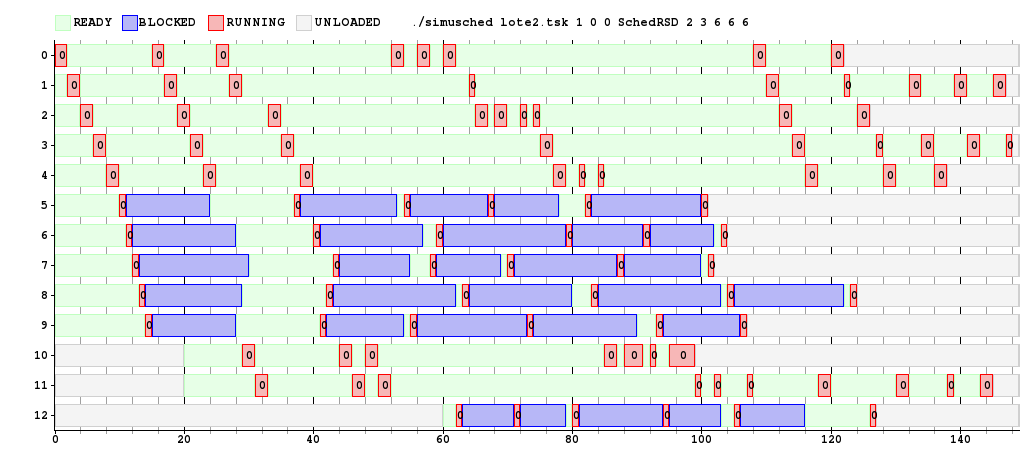
\includegraphics[width=450pt]{./figs/ej91.png}
\end{figure}

Para este experimento se cargaron inicialmente 5 tareas de tipo CPU y 5 de tipo Consola. De acuerdo a lo descrito, el scheduler comienza comportándose cono un $Round$ $Robin$ puesto que todas las tareas comienzan en el mismo nivel. En el tick 20 se cargan otras dos tareas de consola, y se ve claramente cómo estas no van al tope de la prioridad como pasaba al inicio sino que se encolan detrás de las tareas 0 y 1 en el nivel activo, ejecutándose recién alrededor del tick 29. Por otro lado se puede apreciar como alrededor del tick 40 las primeras 5 tareas de consola ya han sufrido un descenso de nivel (pues agotaron su cuota individual) con lo cual sólo las tareas interactivas y las dos últimas de consola agregadas tiempo después permanecen en el nivel de mayor prioridad. En el tick 60 se suma otra tarea de consola, no obstante esta no va a parar al nivel de mayor prioridad puesto que no es el activo en ese momento, por eso sigue en la fila de ejecución de menor prioridad. A partir de este momento se ve de manera definida como sólo las primeras tareas de consola permanecen en el nivel superior, hecho por el cual ni bien se desbloquean son puestas a ejecutar (salvo que justo hubiera otra ejecutando). Más adelante en el tiempo se observa que la prioridad la tienen las tareas interactivas, y que sólo en momentos en que todas están bloqueadas se procede a ejecutar el resto. Este defasaje se nota a lo largo de todo el gráfico, y no sólo entre las de consola y cpu, sino también entre las primeras TaskConsola y las últimas cargadas, las cuales llevan una ventaja de prioridad por sobre las otras por haber sido cargadas después y haber consumido, en cada nivel, menos cuota individual. Eventualmente todas se ejecutan, y aún habiendo tareas en niveles de prioridad superior, si estas están bloqueadas el nivel activo pasará a ser uno de menor prioridad, como se vio en esta explicación, motivo por el cual además de interactivo el algoritmo presenta una buena medida de $fairness$.
